
Table \ref{tab:risk} shows the risk difference and the relative risk of feature variables when compared against the target.
The variable with the highest risk difference is \emph{thalassemia = 2}, with a difference of $0.5203$; meaning, on average, in a sample of $100$ patients $52$ more patients who have Thalassemia (a blood disease characterized by low hemoglobin production) as a fixed defect will develop heart disease than patients without Thalassemia.
The variable with the lowest risk difference is is \emph{thalassemia = 3} with a difference of $-0.4894$; meaning, on average, in a sample of $100$ patients $49$ fewer patients who have Thalassemia as a reversible defect will develop heart disease than patients without Thalassemia. 
Comparing the risk difference to the risk ratio, variables with risk differences less than zero have risk ratios less than 1 and variables with risk differences greater than zero have risk ratios greater than 1. 
\begin{table*}[!bp]
    \caption{Risk Difference and Risk Ratio of Binary Variables} 
    \label{tab:risk}
    \colorbox{gray!20}{
    \resizebox{\textwidth}{!}{
        \begin{tabular}{lrrr}
        \toprule
        {} & Risk Difference & Risk Ratio & RR 95\% Confidence Interval \\
        \midrule
        age                               &         -0.2892 &     0.5671 &          (0.5008, 0.6423)^* \\
        sex                               &         -0.3036 &     0.5809 &          (0.5204, 0.6484)^* \\
        resting blood pressure $>$ 130      &         -0.0888 &      0.839 &          (0.7411, 0.9499)^* \\
        serum cholestoral $>$ 250 ml/dl     &         -0.1512 &     0.7374 &          (0.6473, 0.8401)^* \\
        fasting blood sugar $>$ 120 mg/dl   &         -0.0577 &     0.8893 &           (0.7415, 1.0666) \\
        maximum heart rate achieved $>$ 150 &          0.4067 &      2.364 &          (2.0403, 2.7391)^* \\
        exercise induced angina           &         -0.4633 &     0.3076 &          (0.2483, 0.3809)^* \\
        oldpeak                           &         -0.3773 &      0.435 &          (0.3708, 0.5103)^* \\
        chest pain = 1                    &          0.3455 &     1.7563 &          (1.5815, 1.9503)^* \\
        chest pain = 2                    &          0.3568 &     1.8613 &          (1.6732, 2.0704)^* \\
        chest pain = 3                    &          0.1613 &     1.3219 &          (1.1134, 1.5694)^* \\
        resting electrocardiograph = 1    &          0.1785 &     1.4212 &          (1.2566, 1.6073)^* \\
        resting electrocardiograph = 2    &         -0.3178 &     0.3862 &           (0.1401, 1.0646) \\
        slope = 1                         &         -0.3499 &     0.4837 &          (0.4203, 0.5566)^* \\
        slope = 2                         &          0.3904 &      2.167 &          (1.9032, 2.4674)^* \\
        major vessels colored = 1         &         -0.2837 &     0.5073 &          (0.4105, 0.6268)^* \\
        major vessels colored = 2         &         -0.4101 &     0.2765 &          (0.1859, 0.4112)^* \\
        major vessels colored = 3         &         -0.4104 &     0.2412 &          (0.1308, 0.4448)^* \\
        major vessels colored = 4         &          0.3259 &     1.6422 &           (1.324, 2.0369)^* \\
        thal = 1                          &         -0.1974 &     0.6244 &          (0.4375, 0.8911)^* \\
        thal = 2                          &          0.5203 &     3.1955 &          (2.7033, 3.7772)^* \\
        thal = 3                          &         -0.4894 &     0.3096 &          (0.2562, 0.3742)^* \\
        \bottomrule
        \end{tabular}
    }}
\end{table*}
Of the 22 risk ratios, only 2 variables have confidence intervals that contain 1, and thus accept the null-hypothesis. 
The variable with the highest statistically significant risk ratio is \emph{thalassemia = 2}, with a risk ratio of $3.1955$; meaning, patients who have Thalassemia as a fixed defect are $3.1955$ times more likely to develop heart disease than patients without Thalassemia.
The variable with the lowest statistically significant risk ratio is \emph{major vessels colored = 3}, with a risk ratio of $0.2412$; meaning, patients who had 3 major blood vessels colored in a flourosopy are $0.2412$ times less likely to develop heart disease than patients who had no major blood vessels colored in a flourosopy.


To compute the odds ratios and the marginal effects, a logistic regression model was fit.
\begin{table*}[!tp]
\small
\colorbox{gray!20}{
    \resizebox{\textwidth}{!}{
        \begin{tabular}{c}
        \toprule
        \begin{tabular*}{\textwidth}{lr @{\extracolsep{\fill}} lr}
        \textbf{Dep. Variable:}   &      target      & \textbf{  No. Observations:  } &      615    \\
        \textbf{Model:}           &      Logit       & \textbf{  Df Residuals:      } &      593    \\
        \textbf{Method:}          &       MLE        & \textbf{  Df Model:          } &       21    \\
        \textbf{Date:}            & Mon, 28 Nov 2022 & \textbf{  Pseudo R-squ.:     } &   0.5868    \\
        \textbf{Time:}            &     20:02:19     & \textbf{  Log-Likelihood:    } &   -175.99   \\
        \textbf{converged:}       &       True       & \textbf{  LL-Null:           } &   -425.93   \\
        \textbf{Covariance Type:} &    nonrobust     & \textbf{  LLR p-value:       } & 1.574e-92   \\
        \end{tabular*}    \\
        \bottomrule
        
        \begin{tabular*}{\textwidth}{l  @{\extracolsep{\fill}} rrrrrr}
                            & \textbf{coef} & \textbf{std err} & \textbf{z} & \textbf{P$> |$z$|$} & \textbf{[0.025} & \textbf{0.975]}  \\
        \midrule
        
        \textbf{age}                               &       0.0376  &        0.018     &     2.080  &         0.038        &        0.002    &        0.073     \\
        \textbf{sex}                               &      -2.2499  &        0.433     &    -5.195  &         0.000        &       -3.099    &       -1.401     \\
        \textbf{resting blood pressure}            &      -0.0244  &        0.009     &    -2.857  &         0.004        &       -0.041    &       -0.008     \\
        \textbf{serum cholesterol}                 &      -0.0145  &        0.004     &    -3.853  &         0.000        &       -0.022    &       -0.007     \\
        \textbf{fasting blood sugar $>$ 120 mg/dl} &       0.2915  &        0.441     &     0.661  &         0.509        &       -0.573    &        1.156     \\
        \textbf{maximum heart rate achieved}       &       0.0242  &        0.008     &     2.953  &         0.003        &        0.008    &        0.040     \\
        \textbf{exercise induced angina}           &      -0.4887  &        0.321     &    -1.523  &         0.128        &       -1.118    &        0.140     \\
        \textbf{oldpeak}                           &      -0.5662  &        0.177     &    -3.206  &         0.001        &       -0.912    &       -0.220     \\
        \textbf{chest pain = 1}                    &       0.9770  &        0.421     &     2.320  &         0.020        &        0.152    &        1.802     \\
        \textbf{chest pain = 2}                    &       1.8772  &        0.380     &     4.942  &         0.000        &        1.133    &        2.622     \\
        \textbf{chest pain = 3}                    &       2.4143  &        0.497     &     4.854  &         0.000        &        1.439    &        3.389     \\
        \textbf{resting electrocardiograph = 1}    &       0.1241  &        0.286     &     0.434  &         0.664        &       -0.436    &        0.685     \\
        \textbf{resting electrocardiograph = 2}    &      -0.9711  &        3.222     &    -0.301  &         0.763        &       -7.286    &        5.344     \\
        \textbf{slope = 1}                         &      -0.6824  &        0.610     &    -1.118  &         0.264        &       -1.879    &        0.514     \\
        \textbf{slope = 2}                         &       0.8047  &        0.657     &     1.224  &         0.221        &       -0.484    &        2.093     \\
        \textbf{major vessels colored = 1}         &      -2.4127  &        0.394     &    -6.126  &         0.000        &       -3.185    &       -1.641     \\
        \textbf{major vessels colored = 2}         &      -3.3407  &        0.553     &    -6.041  &         0.000        &       -4.425    &       -2.257     \\
        \textbf{major vessels colored = 3}         &      -2.3139  &        0.697     &    -3.319  &         0.001        &       -3.680    &       -0.947     \\
        \textbf{major vessels colored = 4}         &       1.2003  &        1.213     &     0.990  &         0.322        &       -1.177    &        3.577     \\
        \textbf{thalassemia = 1}                   &       4.1461  &        1.976     &     2.098  &         0.036        &        0.273    &        8.019     \\
        \textbf{thalassemia = 2}                   &       3.9308  &        1.967     &     1.999  &         0.046        &        0.076    &        7.785     \\
        \textbf{thalassemia = 3}                   &       2.6183  &        1.976     &     1.325  &         0.185        &       -1.255    &        6.492     \\

        \end{tabular*}  \\
        \bottomrule
        \end{tabular}
    }
}

\caption{Logistic Regression Results}\label{tab:logit-regression}
\end{table*}
Table~\ref{tab:logit-regression} shows the regression results using the maximum likelihood method.
The log-likelihood of the model is $-175.99$, which is significantly larger than the log-likelihood of the null-model, $-425.93$, given the log-likelihood ratio test p-value of $1.574\mathrm{e-}92$.

Table \ref{tab:odds} shows the odds ratios of the regression, which were obtained by exponentiating the coefficients in table \ref{tab:logit-regression}.
Of the 22 odds ratios, 8 variables have confidence intervals that contain 1, and thus accept the null-hypothesis.
The variable with the highest statistically significant odds ratio is \emph{thalassemia = 1}, with an odds ratio of $63.1862$; meaning, the odds of contacting heart disease are $63.1862$ times higher for patients with normal Thalassemia than patients without Thalassemia.
The variable with the lowest statistically significant odds ratio is \emph{major vessels colored = 2}, with an odds ratio of $0.0354$; meaning, the odds of contacting heart disease are $0.0354$ times lower for patients who had two major blood vessels colored by a fluoroscopy than patients who had no major blood vessels colored by a fluoroscopy.
\def\arraystretch{0.5}
\begin{wraptable}{r}{.55\textwidth}
% \begin{table^^*}[h]
% \small
\centering\caption{Odds Ratios}\label{tab:odds}
\colorbox{gray!20}{
\resizebox{.5\textwidth}{!}{
    \begin{tabular}{lrr}
    \toprule
    {} &  Odds Ratio & OR 95\% Confidence Interval \\
    \midrule
    age       &      1.0383 &          (1.0022, 1.0758)^* \\
    sex       &      0.1054 &          (0.0451, 0.2463)^* \\
    trestbps  &      0.9759 &          (0.9597, 0.9924)^* \\
    chol      &      0.9856 &          (0.9784, 0.9929)^* \\
    fbs       &      1.3384 &           (0.5639, 3.1764) \\
    thalach   &      1.0245 &          (1.0082, 1.0411)^* \\
    exang     &      0.6134 &           (0.3271, 1.1505) \\
    oldpeak   &      0.5677 &          (0.4016, 0.8025)^* \\
    cp\_1      &      2.6565 &          (1.1638, 6.0638)^* \\
    cp\_2      &      6.5352 &          (3.104, 13.7594)^* \\
    cp\_3      &     11.1815 &         (4.2184, 29.6385)^* \\
    restecg\_1 &      1.1322 &           (0.6464, 1.9829) \\
    restecg\_2 &      0.3787 &         (0.0007, 209.2937) \\
    slope\_1   &      0.5054 &           (0.1528, 1.6717) \\
    slope\_2   &      2.2360 &           (0.6163, 8.1119) \\
    ca\_1      &      0.0896 &          (0.0414, 0.1938)^* \\
    ca\_2      &      0.0354 &           (0.012, 0.1047)^* \\
    ca\_3      &      0.0989 &          (0.0252, 0.3878)^* \\
    ca\_4      &      3.3210 &          (0.3082, 35.7816) \\
    thal\_1    &     63.1862 &       (1.3143, 3037.8507)^* \\
    thal\_2    &     50.9487 &       (1.0792, 2405.3763)^* \\
    thal\_3    &     13.7129 &          (0.285, 659.8043) \\
    \bottomrule
    \end{tabular}
}
}
% \end{table^^*}
\end{wraptable}


Table \ref{tab:marginal} shows the marginal effects of the regression output. Of the 22 marginal effects, 8 variables have p-values greater than $5\%$, and thus accept the null-hypothesis. 
It's important to note that these are the same variables that have statistically insignificant odds ratios.
The variable with the highest statistically significant marginal effect is \emph{thalassemia = 1}, with an average marginal effect of $0.3661$; meaning that the average change in probability is $0.3661$ when a patient has normal Thalassemia.
\def\arraystretch{1}
\begin{table*}[!tp]

\small
\colorbox{gray!20}{
    \resizebox{\textwidth}{!}{
    \begin{tabular}{c}
        \toprule
    \begin{tabular*}{\textwidth}{lc}
        \textbf{Dep. Variable:} &     target      \\
        \textbf{Method:}        &      dydx       \\
        \textbf{At:}            &    overall      \\
    \end{tabular*} \\
        \bottomrule

\begin{tabular*}{\textwidth}{l @{\extracolsep{\fill}} rrrrrr}
     \textbf{}      & \textbf{dy/dx} & \textbf{std err} & \textbf{z} & \textbf{P$> |$z$|$} & \textbf{[0.025} & \textbf{0.975]}  \\
\midrule

\textbf{age}        &       0.0033   &        0.002     &     2.109  &         0.035        &        0.000    &        0.006     \\
\textbf{sex}        &      -0.1986   &        0.035     &    -5.658  &         0.000        &       -0.267    &       -0.130     \\
\textbf{trestbps}   &      -0.0022   &        0.001     &    -2.915  &         0.004        &       -0.004    &       -0.001     \\
\textbf{chol}       &      -0.0013   &        0.000     &    -4.070  &         0.000        &       -0.002    &       -0.001     \\
\textbf{fbs}        &       0.0257   &        0.039     &     0.662  &         0.508        &       -0.050    &        0.102     \\
\textbf{thalach}    &       0.0021   &        0.001     &     3.038  &         0.002        &        0.001    &        0.004     \\
\textbf{exang}      &      -0.0431   &        0.028     &    -1.533  &         0.125        &       -0.098    &        0.012     \\
\textbf{oldpeak}    &      -0.0500   &        0.015     &    -3.324  &         0.001        &       -0.079    &       -0.021     \\
\textbf{cp\_1}      &       0.0863   &        0.036     &     2.378  &         0.017        &        0.015    &        0.157     \\
\textbf{cp\_2}      &       0.1657   &        0.031     &     5.338  &         0.000        &        0.105    &        0.227     \\
\textbf{cp\_3}      &       0.2132   &        0.041     &     5.210  &         0.000        &        0.133    &        0.293     \\
\textbf{restecg\_1} &       0.0110   &        0.025     &     0.434  &         0.664        &       -0.039    &        0.060     \\
\textbf{restecg\_2} &      -0.0857   &        0.284     &    -0.301  &         0.763        &       -0.643    &        0.472     \\
\textbf{slope\_1}   &      -0.0602   &        0.054     &    -1.122  &         0.262        &       -0.166    &        0.045     \\
\textbf{slope\_2}   &       0.0710   &        0.058     &     1.229  &         0.219        &       -0.042    &        0.184     \\
\textbf{ca\_1}      &      -0.2130   &        0.030     &    -7.037  &         0.000        &       -0.272    &       -0.154     \\
\textbf{ca\_2}      &      -0.2949   &        0.043     &    -6.804  &         0.000        &       -0.380    &       -0.210     \\
\textbf{ca\_3}      &      -0.2043   &        0.059     &    -3.447  &         0.001        &       -0.320    &       -0.088     \\
\textbf{ca\_4}      &       0.1060   &        0.107     &     0.991  &         0.322        &       -0.104    &        0.316     \\
\textbf{thal\_1}    &       0.3661   &        0.172     &     2.124  &         0.034        &        0.028    &        0.704     \\
\textbf{thal\_2}    &       0.3470   &        0.172     &     2.022  &         0.043        &        0.011    &        0.683     \\
\textbf{thal\_3}    &       0.2312   &        0.174     &     1.331  &         0.183        &       -0.109    &        0.572     \\

\end{tabular*} \\
    \bottomrule
\end{tabular}
}
}

\caption{Marginal Effects}\label{tab:marginal}
\end{table*}

The variable with the lowest statistically significant marginal effect is \emph{major vessels colored = 2}, with an average marginal effect of $-0.2949$; meaning that the average change in probability is $-0.2949$ when a patient who has two major blood vessels colored by a fluoroscopy.

\begin{figure*}[!tp]
    \centering
    \begin{subfigure}[b]{0.49\textwidth}
        \centering
        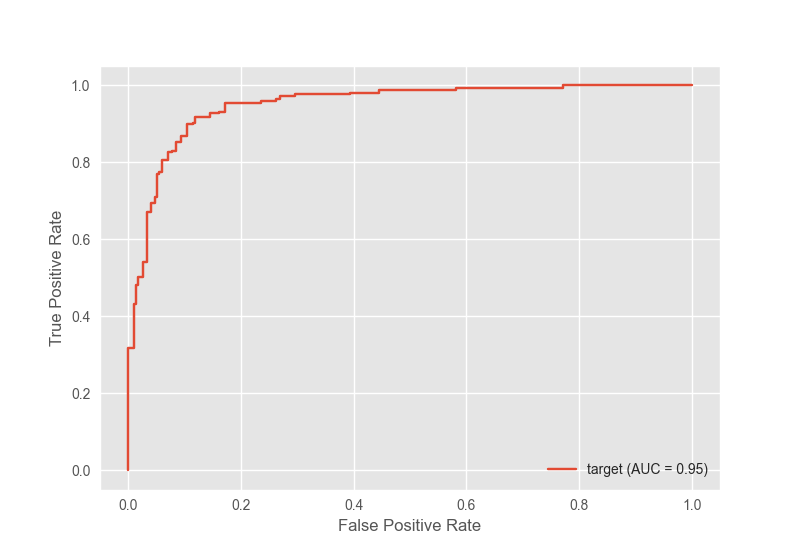
\includegraphics[width=\textwidth]{plots/roc-is-1.png}
        \caption{In Sample}
    \end{subfigure}
    \begin{subfigure}[b]{0.49\textwidth}
        \centering
        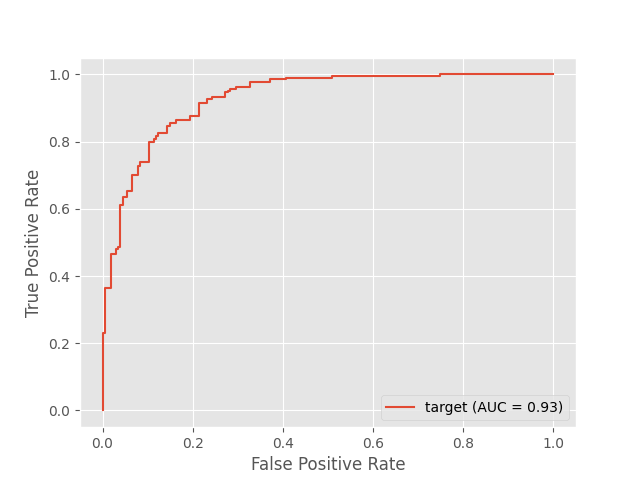
\includegraphics[width=\textwidth]{plots/roc-oos-1.png}
        \caption{Out of Sample}
    \end{subfigure}
    \caption{Receiver Operator Curves}\label{fig:roc}
\end{figure*}
When predicting in sample, the model had a log-loss score of $0.2862$, a Brier score of $0.0836$, and an AUC of $0.9501$, indicating that the model predicts well in sample. 
After training the model, a receiver operating characteristic analysis was applied to determine the optimal threshold for predicting the target. 
To calculate the ROC metrics, a confusion matrix was created for each hundredth between $0$ and $1$. 
The selected threshold was $0.512$ with an accuracy of $0.8943$, a precision of $0.8941$, a sensitivity of $0.9025$, and a specificity of $0.8855$.
When predicting out of sample, the model had a log-loss score of $0.3406$, a Brier score of $0.1073$, and an AUC of $0.9294$, indicating that the model does not lose much generality when introduced to new data. 
Figure~\ref{fig:roc} shows the in sample and out of sample receiver operator curves.


